\documentclass[1p]{elsarticle_modified}
%\bibliographystyle{elsarticle-num}

%\usepackage[colorlinks]{hyperref}
%\usepackage{abbrmath_seonhwa} %\Abb, \Ascr, \Acal ,\Abf, \Afrak
\usepackage{amsfonts}
\usepackage{amssymb}
\usepackage{amsmath}
\usepackage{amsthm}
\usepackage{scalefnt}
\usepackage{amsbsy}
\usepackage{kotex}
\usepackage{caption}
\usepackage{subfig}
\usepackage{color}
\usepackage{graphicx}
\usepackage{xcolor} %% white, black, red, green, blue, cyan, magenta, yellow
\usepackage{float}
\usepackage{setspace}
\usepackage{hyperref}

\usepackage{tikz}
\usetikzlibrary{arrows}

\usepackage{multirow}
\usepackage{array} % fixed length table
\usepackage{hhline}

%%%%%%%%%%%%%%%%%%%%%
\makeatletter
\renewcommand*\env@matrix[1][\arraystretch]{%
	\edef\arraystretch{#1}%
	\hskip -\arraycolsep
	\let\@ifnextchar\new@ifnextchar
	\array{*\c@MaxMatrixCols c}}
\makeatother %https://tex.stackexchange.com/questions/14071/how-can-i-increase-the-line-spacing-in-a-matrix
%%%%%%%%%%%%%%%

\usepackage[normalem]{ulem}

\newcommand{\msout}[1]{\ifmmode\text{\sout{\ensuremath{#1}}}\else\sout{#1}\fi}
%SOURCE: \msout is \stkout macro in https://tex.stackexchange.com/questions/20609/strikeout-in-math-mode

\newcommand{\cancel}[1]{
	\ifmmode
	{\color{red}\msout{#1}}
	\else
	{\color{red}\sout{#1}}
	\fi
}

\newcommand{\add}[1]{
	{\color{blue}\uwave{#1}}
}

\newcommand{\replace}[2]{
	\ifmmode
	{\color{red}\msout{#1}}{\color{blue}\uwave{#2}}
	\else
	{\color{red}\sout{#1}}{\color{blue}\uwave{#2}}
	\fi
}

\newcommand{\Sol}{\mathcal{S}} %segment
\newcommand{\D}{D} %diagram
\newcommand{\A}{\mathcal{A}} %arc


%%%%%%%%%%%%%%%%%%%%%%%%%%%%%5 test

\def\sl{\operatorname{\textup{SL}}(2,\Cbb)}
\def\psl{\operatorname{\textup{PSL}}(2,\Cbb)}
\def\quan{\mkern 1mu \triangleright \mkern 1mu}

\theoremstyle{definition}
\newtheorem{thm}{Theorem}[section]
\newtheorem{prop}[thm]{Proposition}
\newtheorem{lem}[thm]{Lemma}
\newtheorem{ques}[thm]{Question}
\newtheorem{cor}[thm]{Corollary}
\newtheorem{defn}[thm]{Definition}
\newtheorem{exam}[thm]{Example}
\newtheorem{rmk}[thm]{Remark}
\newtheorem{alg}[thm]{Algorithm}

\newcommand{\I}{\sqrt{-1}}
\begin{document}

%\begin{frontmatter}
%
%\title{Boundary parabolic representations of knots up to 8 crossings}
%
%%% Group authors per affiliation:
%\author{Yunhi Cho} 
%\address{Department of Mathematics, University of Seoul, Seoul, Korea}
%\ead{yhcho@uos.ac.kr}
%
%
%\author{Seonhwa Kim} %\fnref{s_kim}}
%\address{Center for Geometry and Physics, Institute for Basic Science, Pohang, 37673, Korea}
%\ead{ryeona17@ibs.re.kr}
%
%\author{Hyuk Kim}
%\address{Department of Mathematical Sciences, Seoul National University, Seoul 08826, Korea}
%\ead{hyukkim@snu.ac.kr}
%
%\author{Seokbeom Yoon}
%\address{Department of Mathematical Sciences, Seoul National University, Seoul, 08826,  Korea}
%\ead{sbyoon15@snu.ac.kr}
%
%\begin{abstract}
%We find all boundary parabolic representation of knots up to 8 crossings.
%
%\end{abstract}
%\begin{keyword}
%    \MSC[2010] 57M25 
%\end{keyword}
%
%\end{frontmatter}

%\linenumbers
%\tableofcontents
%
\newcommand\colored[1]{\textcolor{white}{\rule[-0.35ex]{0.8em}{1.4ex}}\kern-0.8em\color{red} #1}%
%\newcommand\colored[1]{\textcolor{white}{ #1}\kern-2.17ex	\textcolor{white}{ #1}\kern-1.81ex	\textcolor{white}{ #1}\kern-2.15ex\color{red}#1	}

{\Large $\underline{12a_{0682}~(K12a_{0682})}$}

\setlength{\tabcolsep}{10pt}
\renewcommand{\arraystretch}{1.6}
\vspace{1cm}\begin{tabular}{m{100pt}>{\centering\arraybackslash}m{274pt}}
\multirow{5}{120pt}{
	\centering
	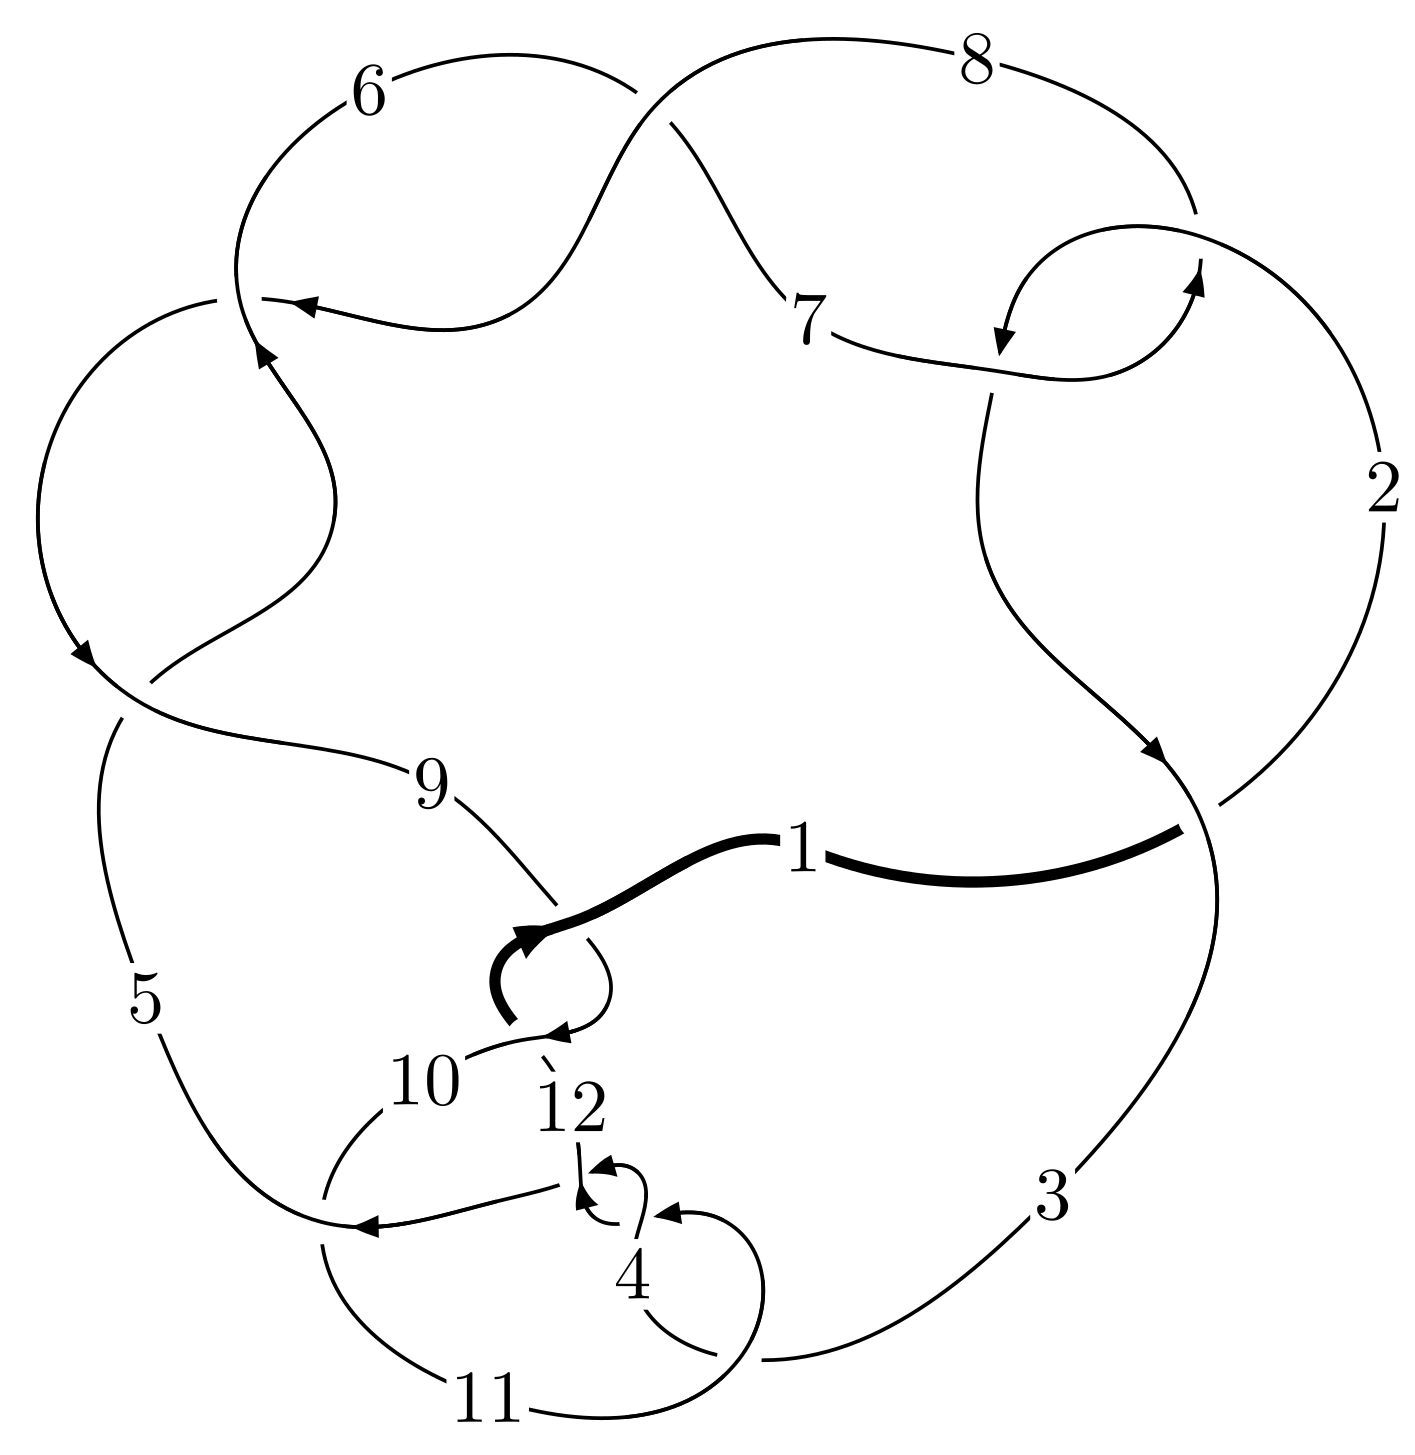
\includegraphics[width=112pt]{../../../GIT/diagram.site/Diagrams/png/1483_12a_0682.png}\\
\ \ \ A knot diagram\footnotemark}&
\allowdisplaybreaks
\textbf{Linearized knot diagam} \\
\cline{2-2}
 &
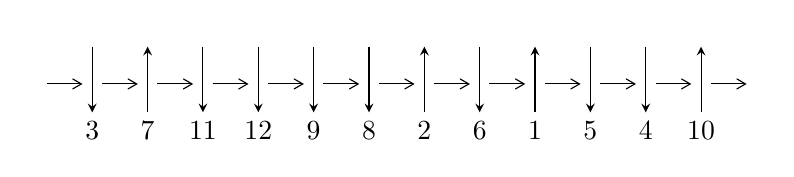
\begin{tikzpicture}[x=20pt, y=17pt]
	% nodes
	\node (C0) at (0, 0) {};
	\node (C1) at (1, 0) {};
	\node (C1U) at (1, +1) {};
	\node (C1D) at (1, -1) {3};

	\node (C2) at (2, 0) {};
	\node (C2U) at (2, +1) {};
	\node (C2D) at (2, -1) {7};

	\node (C3) at (3, 0) {};
	\node (C3U) at (3, +1) {};
	\node (C3D) at (3, -1) {11};

	\node (C4) at (4, 0) {};
	\node (C4U) at (4, +1) {};
	\node (C4D) at (4, -1) {12};

	\node (C5) at (5, 0) {};
	\node (C5U) at (5, +1) {};
	\node (C5D) at (5, -1) {9};

	\node (C6) at (6, 0) {};
	\node (C6U) at (6, +1) {};
	\node (C6D) at (6, -1) {8};

	\node (C7) at (7, 0) {};
	\node (C7U) at (7, +1) {};
	\node (C7D) at (7, -1) {2};

	\node (C8) at (8, 0) {};
	\node (C8U) at (8, +1) {};
	\node (C8D) at (8, -1) {6};

	\node (C9) at (9, 0) {};
	\node (C9U) at (9, +1) {};
	\node (C9D) at (9, -1) {1};

	\node (C10) at (10, 0) {};
	\node (C10U) at (10, +1) {};
	\node (C10D) at (10, -1) {5};

	\node (C11) at (11, 0) {};
	\node (C11U) at (11, +1) {};
	\node (C11D) at (11, -1) {4};

	\node (C12) at (12, 0) {};
	\node (C12U) at (12, +1) {};
	\node (C12D) at (12, -1) {10};
	\node (C13) at (13, 0) {};

	% arrows
	\draw[->,>={angle 60}]
	(C0) edge (C1) (C1) edge (C2) (C2) edge (C3) (C3) edge (C4) (C4) edge (C5) (C5) edge (C6) (C6) edge (C7) (C7) edge (C8) (C8) edge (C9) (C9) edge (C10) (C10) edge (C11) (C11) edge (C12) (C12) edge (C13) ;	\draw[->,>=stealth]
	(C1U) edge (C1D) (C2D) edge (C2U) (C3U) edge (C3D) (C4U) edge (C4D) (C5U) edge (C5D) (C6U) edge (C6D) (C7D) edge (C7U) (C8U) edge (C8D) (C9D) edge (C9U) (C10U) edge (C10D) (C11U) edge (C11D) (C12D) edge (C12U) ;
	\end{tikzpicture} \\
\hhline{~~} \\& 
\textbf{Solving Sequence} \\ \cline{2-2} 
 &
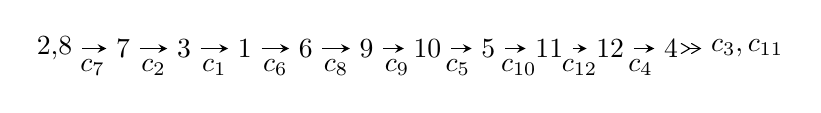
\begin{tikzpicture}[x=22pt, y=7pt]
	% node
	\node (A0) at (-1/8, 0) {2,8};
	\node (A1) at (1, 0) {7};
	\node (A2) at (2, 0) {3};
	\node (A3) at (3, 0) {1};
	\node (A4) at (4, 0) {6};
	\node (A5) at (5, 0) {9};
	\node (A6) at (6, 0) {10};
	\node (A7) at (7, 0) {5};
	\node (A8) at (8, 0) {11};
	\node (A9) at (9, 0) {12};
	\node (A10) at (10, 0) {4};
	\node (C1) at (1/2, -1) {$c_{7}$};
	\node (C2) at (3/2, -1) {$c_{2}$};
	\node (C3) at (5/2, -1) {$c_{1}$};
	\node (C4) at (7/2, -1) {$c_{6}$};
	\node (C5) at (9/2, -1) {$c_{8}$};
	\node (C6) at (11/2, -1) {$c_{9}$};
	\node (C7) at (13/2, -1) {$c_{5}$};
	\node (C8) at (15/2, -1) {$c_{10}$};
	\node (C9) at (17/2, -1) {$c_{12}$};
	\node (C10) at (19/2, -1) {$c_{4}$};
	\node (A11) at (45/4, 0) {$c_{3},c_{11}$};

	% edge
	\draw[->,>=stealth]	
	(A0) edge (A1) (A1) edge (A2) (A2) edge (A3) (A3) edge (A4) (A4) edge (A5) (A5) edge (A6) (A6) edge (A7) (A7) edge (A8) (A8) edge (A9) (A9) edge (A10) ;
	\draw[->>,>={angle 60}]	
	(A10) edge (A11);
\end{tikzpicture} \\ 

\end{tabular} \\

\footnotetext{
The image of knot diagram is generated by the software ``\textbf{Draw programme}" developed by Andrew Bartholomew(\url{http://www.layer8.co.uk/maths/draw/index.htm\#Running-draw}), where we modified some parts for our purpose(\url{https://github.com/CATsTAILs/LinksPainter}).
}\phantom \\ \newline 
\centering \textbf{Ideals for irreducible components\footnotemark of $X_{\text{par}}$} 
 
\begin{align*}
I^u_{1}&=\langle 
u^{53}+u^{52}+\cdots+u+1\rangle \\
\\
\end{align*}
\raggedright * 1 irreducible components of $\dim_{\mathbb{C}}=0$, with total 53 representations.\\
\footnotetext{All coefficients of polynomials are rational numbers. But the coefficients are sometimes approximated in decimal forms when there is not enough margin.}
\newpage
\renewcommand{\arraystretch}{1}
\centering \section*{I. $I^u_{1}= \langle u^{53}+u^{52}+\cdots+u+1 \rangle$}
\flushleft \textbf{(i) Arc colorings}\\
\begin{tabular}{m{7pt} m{180pt} m{7pt} m{180pt} }
\flushright $a_{2}=$&$\begin{pmatrix}0\\u\end{pmatrix}$ \\
\flushright $a_{8}=$&$\begin{pmatrix}1\\0\end{pmatrix}$ \\
\flushright $a_{7}=$&$\begin{pmatrix}1\\u^2\end{pmatrix}$ \\
\flushright $a_{3}=$&$\begin{pmatrix}u\\u^3+u\end{pmatrix}$ \\
\flushright $a_{1}=$&$\begin{pmatrix}u^3\\u^5+u^3+u\end{pmatrix}$ \\
\flushright $a_{6}=$&$\begin{pmatrix}u^2+1\\u^2\end{pmatrix}$ \\
\flushright $a_{9}=$&$\begin{pmatrix}u^4+u^2+1\\u^4\end{pmatrix}$ \\
\flushright $a_{10}=$&$\begin{pmatrix}- u^{12}- u^{10}-3 u^8-2 u^6+u^2+1\\- u^{14}-2 u^{12}-5 u^{10}-6 u^8-6 u^6-2 u^4- u^2\end{pmatrix}$ \\
\flushright $a_{5}=$&$\begin{pmatrix}u^6+u^4+2 u^2+1\\u^6+u^2\end{pmatrix}$ \\
\flushright $a_{11}=$&$\begin{pmatrix}u^{26}+3 u^{24}+\cdots+3 u^2+1\\u^{26}+2 u^{24}+\cdots- u^6- u^2\end{pmatrix}$ \\
\flushright $a_{12}=$&$\begin{pmatrix}u^{21}+2 u^{19}+7 u^{17}+10 u^{15}+14 u^{13}+12 u^{11}+5 u^9-2 u^7-5 u^5-2 u^3- u\\u^{23}+3 u^{21}+\cdots+2 u^3+u\end{pmatrix}$ \\
\flushright $a_{4}=$&$\begin{pmatrix}- u^{50}-5 u^{48}+\cdots+3 u^2+1\\- u^{52}-6 u^{50}+\cdots-26 u^6-7 u^4\end{pmatrix}$\\&\end{tabular}
\flushleft \textbf{(ii) Obstruction class $= -1$}\\~\\
\flushleft \textbf{(iii) Cusp Shapes $= -4 u^{51}-4 u^{50}+\cdots-16 u-10$}\\~\\
\newpage\renewcommand{\arraystretch}{1}
\flushleft \textbf{(iv) u-Polynomials at the component}\newline \\
\begin{tabular}{m{50pt}|m{274pt}}
Crossings & \hspace{64pt}u-Polynomials at each crossing \\
\hline $$\begin{aligned}c_{1},c_{5},c_{6}\\c_{8}\end{aligned}$$&$\begin{aligned}
&u^{53}+11 u^{52}+\cdots-5 u-1
\end{aligned}$\\
\hline $$\begin{aligned}c_{2},c_{7}\end{aligned}$$&$\begin{aligned}
&u^{53}+u^{52}+\cdots+u+1
\end{aligned}$\\
\hline $$\begin{aligned}c_{3},c_{4},c_{11}\end{aligned}$$&$\begin{aligned}
&u^{53}+u^{52}+\cdots+3 u+1
\end{aligned}$\\
\hline $$\begin{aligned}c_{9},c_{12}\end{aligned}$$&$\begin{aligned}
&u^{53}+9 u^{52}+\cdots+857 u+89
\end{aligned}$\\
\hline $$\begin{aligned}c_{10}\end{aligned}$$&$\begin{aligned}
&u^{53}-3 u^{52}+\cdots-179 u-105
\end{aligned}$\\
\hline
\end{tabular}\\~\\
\newpage\renewcommand{\arraystretch}{1}
\flushleft \textbf{(v) Riley Polynomials at the component}\newline \\
\begin{tabular}{m{50pt}|m{274pt}}
Crossings & \hspace{64pt}Riley Polynomials at each crossing \\
\hline $$\begin{aligned}c_{1},c_{5},c_{6}\\c_{8}\end{aligned}$$&$\begin{aligned}
&y^{53}+63 y^{52}+\cdots-13 y-1
\end{aligned}$\\
\hline $$\begin{aligned}c_{2},c_{7}\end{aligned}$$&$\begin{aligned}
&y^{53}+11 y^{52}+\cdots-5 y-1
\end{aligned}$\\
\hline $$\begin{aligned}c_{3},c_{4},c_{11}\end{aligned}$$&$\begin{aligned}
&y^{53}-49 y^{52}+\cdots-5 y-1
\end{aligned}$\\
\hline $$\begin{aligned}c_{9},c_{12}\end{aligned}$$&$\begin{aligned}
&y^{53}+35 y^{52}+\cdots-196313 y-7921
\end{aligned}$\\
\hline $$\begin{aligned}c_{10}\end{aligned}$$&$\begin{aligned}
&y^{53}-13 y^{52}+\cdots+120871 y-11025
\end{aligned}$\\
\hline
\end{tabular}\\~\\
\newpage\flushleft \textbf{(vi) Complex Volumes and Cusp Shapes}
$$\begin{array}{c|c|c}  
\text{Solutions to }I^u_{1}& \I (\text{vol} + \sqrt{-1}CS) & \text{Cusp shape}\\
 \hline 
\begin{aligned}
u &= \phantom{-}0.457945 + 0.892866 I\end{aligned}
 & -1.71286 + 2.75389 I & -6.34294 - 3.07234 I \\ \hline\begin{aligned}
u &= \phantom{-}0.457945 - 0.892866 I\end{aligned}
 & -1.71286 - 2.75389 I & -6.34294 + 3.07234 I \\ \hline\begin{aligned}
u &= \phantom{-}0.572730 + 0.813144 I\end{aligned}
 & -1.00719 + 4.98869 I & -3.18777 - 7.70135 I \\ \hline\begin{aligned}
u &= \phantom{-}0.572730 - 0.813144 I\end{aligned}
 & -1.00719 - 4.98869 I & -3.18777 + 7.70135 I \\ \hline\begin{aligned}
u &= -0.429825 + 0.920962 I\end{aligned}
 & -7.86744 - 0.15769 I & -10.16108 + 3.00425 I \\ \hline\begin{aligned}
u &= -0.429825 - 0.920962 I\end{aligned}
 & -7.86744 + 0.15769 I & -10.16108 - 3.00425 I \\ \hline\begin{aligned}
u &= -0.490682 + 0.914221 I\end{aligned}
 & -1.20646 - 6.61760 I & -4.55514 + 9.49134 I \\ \hline\begin{aligned}
u &= -0.490682 - 0.914221 I\end{aligned}
 & -1.20646 + 6.61760 I & -4.55514 - 9.49134 I \\ \hline\begin{aligned}
u &= \phantom{-}0.493153 + 0.936516 I\end{aligned}
 & -7.05643 + 9.90285 I & -8.45292 - 8.93815 I \\ \hline\begin{aligned}
u &= \phantom{-}0.493153 - 0.936516 I\end{aligned}
 & -7.05643 - 9.90285 I & -8.45292 + 8.93815 I \\ \hline\begin{aligned}
u &= -0.036116 + 0.938626 I\end{aligned}
 & -10.01760 - 4.89958 I & -13.7857 + 3.6935 I \\ \hline\begin{aligned}
u &= -0.036116 - 0.938626 I\end{aligned}
 & -10.01760 + 4.89958 I & -13.7857 - 3.6935 I \\ \hline\begin{aligned}
u &= -0.575852 + 0.733397 I\end{aligned}
 & \phantom{-}2.95450 - 2.17059 I & \phantom{-}3.89779 + 4.69702 I \\ \hline\begin{aligned}
u &= -0.575852 - 0.733397 I\end{aligned}
 & \phantom{-}2.95450 + 2.17059 I & \phantom{-}3.89779 - 4.69702 I \\ \hline\begin{aligned}
u &= \phantom{-}0.023560 + 0.907629 I\end{aligned}
 & -4.02491 + 1.91090 I & -10.66650 - 3.96746 I \\ \hline\begin{aligned}
u &= \phantom{-}0.023560 - 0.907629 I\end{aligned}
 & -4.02491 - 1.91090 I & -10.66650 + 3.96746 I \\ \hline\begin{aligned}
u &= \phantom{-}0.610238 + 0.641474 I\end{aligned}
 & -0.472073 - 0.554107 I & -1.056775 + 0.178286 I \\ \hline\begin{aligned}
u &= \phantom{-}0.610238 - 0.641474 I\end{aligned}
 & -0.472073 + 0.554107 I & -1.056775 - 0.178286 I \\ \hline\begin{aligned}
u &= -0.217456 + 0.806943 I\end{aligned}
 & -4.96706 - 2.01723 I & -11.79175 + 5.17722 I \\ \hline\begin{aligned}
u &= -0.217456 - 0.806943 I\end{aligned}
 & -4.96706 + 2.01723 I & -11.79175 - 5.17722 I \\ \hline\begin{aligned}
u &= \phantom{-}0.661436 + 0.434620 I\end{aligned}
 & -5.46999 - 5.61580 I & -4.48224 + 3.23992 I \\ \hline\begin{aligned}
u &= \phantom{-}0.661436 - 0.434620 I\end{aligned}
 & -5.46999 + 5.61580 I & -4.48224 - 3.23992 I \\ \hline\begin{aligned}
u &= -0.618304 + 0.456294 I\end{aligned}
 & \phantom{-}0.22206 + 2.44713 I & -0.32336 - 3.63578 I \\ \hline\begin{aligned}
u &= -0.618304 - 0.456294 I\end{aligned}
 & \phantom{-}0.22206 - 2.44713 I & -0.32336 + 3.63578 I \\ \hline\begin{aligned}
u &= \phantom{-}0.876686 + 0.875322 I\end{aligned}
 & \phantom{-}0.37975 + 3.02773 I & \phantom{-0.000000 } 0 \\ \hline\begin{aligned}
u &= \phantom{-}0.876686 - 0.875322 I\end{aligned}
 & \phantom{-}0.37975 - 3.02773 I & \phantom{-0.000000 } 0 \\ \hline\begin{aligned}
u &= -0.890877 + 0.888837 I\end{aligned}
 & \phantom{-}6.84069 - 0.89167 I & \phantom{-0.000000 } 0 \\ \hline\begin{aligned}
u &= -0.890877 - 0.888837 I\end{aligned}
 & \phantom{-}6.84069 + 0.89167 I & \phantom{-0.000000 } 0 \\ \hline\begin{aligned}
u &= -0.907804 + 0.877338 I\end{aligned}
 & \phantom{-}2.05866 + 6.62991 I & \phantom{-0.000000 } 0 \\ \hline\begin{aligned}
u &= -0.907804 - 0.877338 I\end{aligned}
 & \phantom{-}2.05866 - 6.62991 I & \phantom{-0.000000 } 0\\
 \hline 
 \end{array}$$\newpage$$\begin{array}{c|c|c}  
\text{Solutions to }I^u_{1}& \I (\text{vol} + \sqrt{-1}CS) & \text{Cusp shape}\\
 \hline 
\begin{aligned}
u &= \phantom{-}0.903027 + 0.883843 I\end{aligned}
 & \phantom{-}7.77793 - 3.11403 I & \phantom{-0.000000 } 0 \\ \hline\begin{aligned}
u &= \phantom{-}0.903027 - 0.883843 I\end{aligned}
 & \phantom{-}7.77793 + 3.11403 I & \phantom{-0.000000 } 0 \\ \hline\begin{aligned}
u &= \phantom{-}0.847469 + 0.952356 I\end{aligned}
 & \phantom{-}0.13857 + 3.36391 I & \phantom{-0.000000 } 0 \\ \hline\begin{aligned}
u &= \phantom{-}0.847469 - 0.952356 I\end{aligned}
 & \phantom{-}0.13857 - 3.36391 I & \phantom{-0.000000 } 0 \\ \hline\begin{aligned}
u &= -0.898144 + 0.916667 I\end{aligned}
 & \phantom{-}8.05683 + 0.13889 I & \phantom{-0.000000 } 0 \\ \hline\begin{aligned}
u &= -0.898144 - 0.916667 I\end{aligned}
 & \phantom{-}8.05683 - 0.13889 I & \phantom{-0.000000 } 0 \\ \hline\begin{aligned}
u &= -0.862668 + 0.953089 I\end{aligned}
 & \phantom{-}6.63594 - 5.59402 I & \phantom{-0.000000 } 0 \\ \hline\begin{aligned}
u &= -0.862668 - 0.953089 I\end{aligned}
 & \phantom{-}6.63594 + 5.59402 I & \phantom{-0.000000 } 0 \\ \hline\begin{aligned}
u &= \phantom{-}0.891690 + 0.928721 I\end{aligned}
 & \phantom{-}11.67710 + 3.29120 I & \phantom{-0.000000 } 0 \\ \hline\begin{aligned}
u &= \phantom{-}0.891690 - 0.928721 I\end{aligned}
 & \phantom{-}11.67710 - 3.29120 I & \phantom{-0.000000 } 0 \\ \hline\begin{aligned}
u &= -0.886770 + 0.940938 I\end{aligned}
 & \phantom{-}7.97899 - 6.72566 I & \phantom{-0.000000 } 0 \\ \hline\begin{aligned}
u &= -0.886770 - 0.940938 I\end{aligned}
 & \phantom{-}7.97899 + 6.72566 I & \phantom{-0.000000 } 0 \\ \hline\begin{aligned}
u &= \phantom{-}0.866244 + 0.963279 I\end{aligned}
 & \phantom{-}7.52338 + 9.64804 I & \phantom{-0.000000 } 0 \\ \hline\begin{aligned}
u &= \phantom{-}0.866244 - 0.963279 I\end{aligned}
 & \phantom{-}7.52338 - 9.64804 I & \phantom{-0.000000 } 0 \\ \hline\begin{aligned}
u &= -0.864545 + 0.969690 I\end{aligned}
 & \phantom{-}1.76241 - 13.17230 I & \phantom{-0.000000 } 0 \\ \hline\begin{aligned}
u &= -0.864545 - 0.969690 I\end{aligned}
 & \phantom{-}1.76241 + 13.17230 I & \phantom{-0.000000 } 0 \\ \hline\begin{aligned}
u &= -0.598640 + 0.307693 I\end{aligned}
 & -6.03882 - 3.60466 I & -5.04712 + 3.30603 I \\ \hline\begin{aligned}
u &= -0.598640 - 0.307693 I\end{aligned}
 & -6.03882 + 3.60466 I & -5.04712 - 3.30603 I \\ \hline\begin{aligned}
u &= \phantom{-}0.498225 + 0.373224 I\end{aligned}
 & -0.283096 + 0.992412 I & -1.65563 - 4.45703 I \\ \hline\begin{aligned}
u &= \phantom{-}0.498225 - 0.373224 I\end{aligned}
 & -0.283096 - 0.992412 I & -1.65563 + 4.45703 I \\ \hline\begin{aligned}
u &= \phantom{-}0.297051 + 0.536713 I\end{aligned}
 & -0.193421 + 0.916328 I & -4.23122 - 6.90314 I \\ \hline\begin{aligned}
u &= \phantom{-}0.297051 - 0.536713 I\end{aligned}
 & -0.193421 - 0.916328 I & -4.23122 + 6.90314 I \\ \hline\begin{aligned}
u &= -0.443543\phantom{ +0.000000I}\end{aligned}
 & -2.70485\phantom{ +0.000000I} & -1.55100\phantom{ +0.000000I}\\
 \hline 
 \end{array}$$\newpage
\newpage\renewcommand{\arraystretch}{1}
\centering \section*{ II. u-Polynomials}
\begin{tabular}{m{50pt}|m{274pt}}
Crossings & \hspace{64pt}u-Polynomials at each crossing \\
\hline $$\begin{aligned}c_{1},c_{5},c_{6}\\c_{8}\end{aligned}$$&$\begin{aligned}
&u^{53}+11 u^{52}+\cdots-5 u-1
\end{aligned}$\\
\hline $$\begin{aligned}c_{2},c_{7}\end{aligned}$$&$\begin{aligned}
&u^{53}+u^{52}+\cdots+u+1
\end{aligned}$\\
\hline $$\begin{aligned}c_{3},c_{4},c_{11}\end{aligned}$$&$\begin{aligned}
&u^{53}+u^{52}+\cdots+3 u+1
\end{aligned}$\\
\hline $$\begin{aligned}c_{9},c_{12}\end{aligned}$$&$\begin{aligned}
&u^{53}+9 u^{52}+\cdots+857 u+89
\end{aligned}$\\
\hline $$\begin{aligned}c_{10}\end{aligned}$$&$\begin{aligned}
&u^{53}-3 u^{52}+\cdots-179 u-105
\end{aligned}$\\
\hline
\end{tabular}\newpage\renewcommand{\arraystretch}{1}
\centering \section*{ III. Riley Polynomials}
\begin{tabular}{m{50pt}|m{274pt}}
Crossings & \hspace{64pt}Riley Polynomials at each crossing \\
\hline $$\begin{aligned}c_{1},c_{5},c_{6}\\c_{8}\end{aligned}$$&$\begin{aligned}
&y^{53}+63 y^{52}+\cdots-13 y-1
\end{aligned}$\\
\hline $$\begin{aligned}c_{2},c_{7}\end{aligned}$$&$\begin{aligned}
&y^{53}+11 y^{52}+\cdots-5 y-1
\end{aligned}$\\
\hline $$\begin{aligned}c_{3},c_{4},c_{11}\end{aligned}$$&$\begin{aligned}
&y^{53}-49 y^{52}+\cdots-5 y-1
\end{aligned}$\\
\hline $$\begin{aligned}c_{9},c_{12}\end{aligned}$$&$\begin{aligned}
&y^{53}+35 y^{52}+\cdots-196313 y-7921
\end{aligned}$\\
\hline $$\begin{aligned}c_{10}\end{aligned}$$&$\begin{aligned}
&y^{53}-13 y^{52}+\cdots+120871 y-11025
\end{aligned}$\\
\hline
\end{tabular}
\vskip 2pc
\end{document}